% !TeX root = ../courtade-kumar.tex
\usetikzlibrary{decorations.markings}
% blue/purple scheme
\definecolor{lecol}{RGB}{40,160,235}
\definecolor{gecol}{RGB}{140,82,235}
\def\regionopacity{0.28}
% green/blue scheme (swap in to use; update caption colour names)
% \colorlet{lecol}{green!55!black}
% \colorlet{gecol}{blue!70!black}
% \def\regionopacity{0.18}
\begin{figure}[H]
\centering
\vspace*{0.5em}
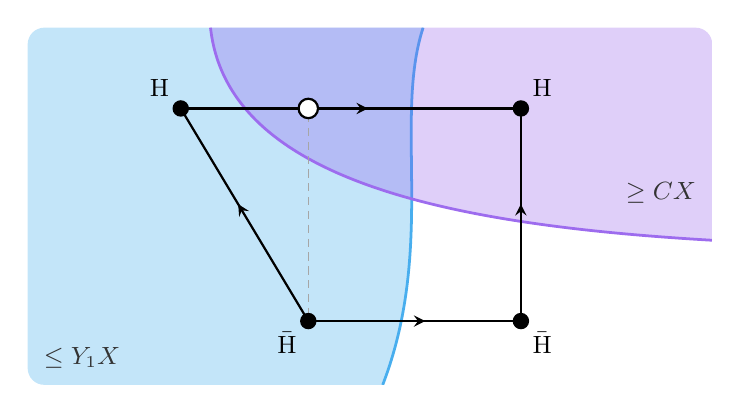
\begin{tikzpicture}[scale=2.7,
    corner/.style={font=\small},
    inc/.style={thick,line cap=round,postaction={decorate},
      decoration={markings,mark=at position 0.55 with {\arrow{stealth}}}}]
  % Top edge \sI H -> \qI H has length (\qI - \sI)H; bottom edge has
  % length (\qI - \sI)\bar H. Q sits on the top edge at distance
  % (\qI - \sI)\bar H from \qI H, i.e. directly above \sI \bar H.
  \coordinate (HI)   at (0,1);
  \coordinate (HbI)  at (1.6,1);
  \coordinate (bHI)  at (0.6,0);
  \coordinate (bHbI) at (1.6,0);
  \coordinate (Q)    at (0.6,1);
  % shaded regions; their overlap blends to a third colour
  \begin{scope}
    \clip[rounded corners=6pt] (-0.72,-0.3) rectangle (2.5,1.38);
    % values guaranteed <= I
    \fill[lecol,opacity=\regionopacity]
      (-0.72,-0.3) -- (0.95,-0.3)
      .. controls (1.2,0.35) and (1.0,0.95) .. (1.14,1.38)
      -- (-0.72,1.38) -- cycle;
    \draw[lecol!85,line width=1pt]
      (0.95,-0.3) .. controls (1.2,0.35) and (1.0,0.95) .. (1.14,1.38);
    % values guaranteed >= I(B:X)
    \fill[gecol,opacity=\regionopacity]
      (0.14,1.38) .. controls (0.22,0.65) and (1.3,0.45) .. (2.5,0.38)
      -- (2.5,1.38) -- cycle;
    \draw[gecol!85,line width=1pt]
      (0.14,1.38) .. controls (0.22,0.65) and (1.3,0.45) .. (2.5,0.38);
  \end{scope}
  \node[black!80,font=\small,anchor=south west] at (-0.69,-0.27)
    {$\le\muti{Y_1}{X}$};
  \node[black!80,font=\small,anchor=north east] at (2.47,0.70)
    {$\ge\muti{C}{X}$};
  % edges point in the increasing direction
  \draw[inc] (HI)   -- (HbI);
  \draw[inc] (bHI)  -- (bHbI);
  \draw[inc] (bHI)  -- (HI);
  \draw[inc] (bHbI) -- (HbI);
  \draw[densely dashed,gray!70,shorten >=2pt,shorten <=2pt] (Q) -- (bHI);
  \foreach \p in {HI,HbI,bHI,bHbI} \fill (\p) circle (1.1pt);
  \filldraw[fill=white,thick] (Q) circle (1.3pt);
  % mid anchors are baseline-relative, so the two top labels share a baseline
  \node[corner,anchor=south east,inner sep=4pt] at (HI)   {$\sI\mathrm H$};
  \node[corner,anchor=south west,inner sep=4pt] at (HbI)  {$\qI\mathrm H$};
  \node[corner,anchor=north east,inner sep=4pt] at (bHI)  {$\sI\bar{\mathrm H}$};
  \node[corner,anchor=north west,inner sep=4pt] at (bHbI) {$\qI\bar{\mathrm H}$};
  \node[anchor=south,inner sep=5pt] at (Q) {$\Q$};
\end{tikzpicture}
\captionsetup{font=small,name=Figure,labelformat=default,labelsep=period,labelfont=bf}
\caption{Arrows point toward the larger quantity.
$\Q$ lies on the top edge, and its distance to
$\qI\ent{C}$ equals the length of the bottom edge,
$(\qI-\sI)\,\tsent{C}$.
Blue: quantities that are always at most $\muti{Y_1}{X}$.
Purple: quantities that upper bound $\muti{C}{X}$.
Only $\Q$ lies in both.}
\label{fig:q-square}
\end{figure}
